% This is the Reed College LaTeX thesis template. Most of the work
% for the document class was done by Sam Noble (SN), as well as this
% template. Later comments etc. by Ben Salzberg (BTS). Additional
% restructuring and APA support by Jess Youngberg (JY).
% Your comments and suggestions are more than welcome; please email
% them to cus@reed.edu
%
% See http://web.reed.edu/cis/help/latex.html for help. There are a
% great bunch of help pages there, with notes on
% getting started, bibtex, etc. Go there and read it if you're not
% already familiar with LaTeX.
%
% Any line that starts with a percent symbol is a comment.
% They won't show up in the document, and are useful for notes
% to yourself and explaining commands.
% Commenting also removes a line from the document;
% very handy for troubleshooting problems. -BTS

% As far as I know, this follows the requirements laid out in
% the 2002-2003 Senior Handbook. Ask a librarian to check the
% document before binding. -SN

%%
%% Preamble
%%
% \documentclass{<something>} must begin each LaTeX document
\documentclass[12pt,twoside,openany]{reedthesis}
% Packages are extensions to the basic LaTeX functions. Whatever you
% want to typeset, there is probably a package out there for it.
% Chemistry (chemtex), screenplays, you name it.
% Check out CTAN to see: http://www.ctan.org/
%%

\usepackage{setspace}
\usepackage{graphicx,latexsym}
\usepackage{amsmath}
\usepackage{amssymb,amsthm}
%\usepackage{longtable,booktabs,setspace}
\usepackage{longtable,booktabs,setspace, array}
\usepackage{chemarr} %% Useful for one reaction arrow, useless if you're not a chem major
\usepackage[hyphens]{url}
% Added by CII
\usepackage{hyperref}
\usepackage{lmodern}
\usepackage{float}
\floatplacement{figure}{H}
% End of CII addition
\usepackage{rotating}
% Next line commented out by CII
%%% \usepackage{natbib}
% Comment out the natbib line above and uncomment the following two lines to use the new
% biblatex-chicago style, for Chicago A. Also make some changes at the end where the
% bibliography is included.
%\usepackage{biblatex-chicago}
%\bibliography{thesis}


% Added by CII (Thanks, Hadley!)
% Use ref for internal links
\renewcommand{\hyperref}[2][???]{\autoref{#1}}
\def\chapterautorefname{Chapter}
\def\sectionautorefname{Section}
\def\subsectionautorefname{Subsection}
% End of CII addition

% Added by CII
\usepackage{caption}
\captionsetup{width=5in}
% End of CII addition

% \usepackage{times} % other fonts are available like times, bookman, charter, palatino

% Syntax highlighting #22
  \usepackage{color}
  \usepackage{fancyvrb}
  \newcommand{\VerbBar}{|}
  \newcommand{\VERB}{\Verb[commandchars=\\\{\}]}
  \DefineVerbatimEnvironment{Highlighting}{Verbatim}{commandchars=\\\{\}}
  % Add ',fontsize=\small' for more characters per line
  \usepackage{framed}
  \definecolor{shadecolor}{RGB}{248,248,248}
  \newenvironment{Shaded}{\begin{snugshade}}{\end{snugshade}}
  \newcommand{\AlertTok}[1]{\textcolor[rgb]{0.94,0.16,0.16}{#1}}
  \newcommand{\AnnotationTok}[1]{\textcolor[rgb]{0.56,0.35,0.01}{\textbf{\textit{#1}}}}
  \newcommand{\AttributeTok}[1]{\textcolor[rgb]{0.77,0.63,0.00}{#1}}
  \newcommand{\BaseNTok}[1]{\textcolor[rgb]{0.00,0.00,0.81}{#1}}
  \newcommand{\BuiltInTok}[1]{#1}
  \newcommand{\CharTok}[1]{\textcolor[rgb]{0.31,0.60,0.02}{#1}}
  \newcommand{\CommentTok}[1]{\textcolor[rgb]{0.56,0.35,0.01}{\textit{#1}}}
  \newcommand{\CommentVarTok}[1]{\textcolor[rgb]{0.56,0.35,0.01}{\textbf{\textit{#1}}}}
  \newcommand{\ConstantTok}[1]{\textcolor[rgb]{0.00,0.00,0.00}{#1}}
  \newcommand{\ControlFlowTok}[1]{\textcolor[rgb]{0.13,0.29,0.53}{\textbf{#1}}}
  \newcommand{\DataTypeTok}[1]{\textcolor[rgb]{0.13,0.29,0.53}{#1}}
  \newcommand{\DecValTok}[1]{\textcolor[rgb]{0.00,0.00,0.81}{#1}}
  \newcommand{\DocumentationTok}[1]{\textcolor[rgb]{0.56,0.35,0.01}{\textbf{\textit{#1}}}}
  \newcommand{\ErrorTok}[1]{\textcolor[rgb]{0.64,0.00,0.00}{\textbf{#1}}}
  \newcommand{\ExtensionTok}[1]{#1}
  \newcommand{\FloatTok}[1]{\textcolor[rgb]{0.00,0.00,0.81}{#1}}
  \newcommand{\FunctionTok}[1]{\textcolor[rgb]{0.00,0.00,0.00}{#1}}
  \newcommand{\ImportTok}[1]{#1}
  \newcommand{\InformationTok}[1]{\textcolor[rgb]{0.56,0.35,0.01}{\textbf{\textit{#1}}}}
  \newcommand{\KeywordTok}[1]{\textcolor[rgb]{0.13,0.29,0.53}{\textbf{#1}}}
  \newcommand{\NormalTok}[1]{#1}
  \newcommand{\OperatorTok}[1]{\textcolor[rgb]{0.81,0.36,0.00}{\textbf{#1}}}
  \newcommand{\OtherTok}[1]{\textcolor[rgb]{0.56,0.35,0.01}{#1}}
  \newcommand{\PreprocessorTok}[1]{\textcolor[rgb]{0.56,0.35,0.01}{\textit{#1}}}
  \newcommand{\RegionMarkerTok}[1]{#1}
  \newcommand{\SpecialCharTok}[1]{\textcolor[rgb]{0.00,0.00,0.00}{#1}}
  \newcommand{\SpecialStringTok}[1]{\textcolor[rgb]{0.31,0.60,0.02}{#1}}
  \newcommand{\StringTok}[1]{\textcolor[rgb]{0.31,0.60,0.02}{#1}}
  \newcommand{\VariableTok}[1]{\textcolor[rgb]{0.00,0.00,0.00}{#1}}
  \newcommand{\VerbatimStringTok}[1]{\textcolor[rgb]{0.31,0.60,0.02}{#1}}
  \newcommand{\WarningTok}[1]{\textcolor[rgb]{0.56,0.35,0.01}{\textbf{\textit{#1}}}}

% To pass between YAML and LaTeX the dollar signs are added by CII
\title{Regime Detection Measures for the Practical Ecologist}
\author{Jessica L. Burnett}
% The month and year that you submit your FINAL draft TO THE LIBRARY
\date{2019}
% \division{}
\advisor{Craig R. Allen}
\department{School of Natural Resources}
\institution{University of Nebraska-Lincoln}
\degree{Doctor of Philosophy}
%If you have two advisors for some reason, you can use the following
% Uncommented out by CII
\altadvisor{Dirac Twidwell}
% End of CII addition

%%% Remember to use the correct department!
% if you're writing a thesis in an interdisciplinary major,
% uncomment the line below and change the text as appropriate.
% check the Senior Handbook if unsure.
%\thedivisionof{The Established Interdisciplinary Committee for}
% if you want the approval page to say "Approved for the Committee",
% uncomment the next line
%\approvedforthe{Committee}

% Added by CII
%%% Copied from knitr
%% maxwidth is the original width if it's less than linewidth
%% otherwise use linewidth (to make sure the graphics do not exceed the margin)
\makeatletter
\def\maxwidth{ %
  \ifdim\Gin@nat@width>\linewidth
    \linewidth
  \else
    \Gin@nat@width
  \fi
}
\makeatother

\renewcommand{\contentsname}{Table of Contents}
% End of CII addition

\setlength{\parskip}{0pt}

% Added by CII

\providecommand{\tightlist}{%
  \setlength{\itemsep}{0pt}\setlength{\parskip}{0pt}}

\Acknowledgements{
Graduate school itself isn't hard, but the journey is. I have a lot of people and institutions to thank for their emotional, intellectual, financial, and other support. I wish to first highlight how \textbf{great it was to be a graduate student at this university and in the School of Natural Resources}. UNL has provided tremendous support at all levels of the university. Although I am not a fan of Nebraska's climate, I highly recommend this school to prospective students.
I thank my supervisors, Craig Allen and Dirac Twidwell, for providing me with this amazing opportunity and for supporting my growth as an independent researcherm and my committee members, Craig Allen, David Angeler, John De Long, Dirac Twidwell, and Drew Tyre for their support and advisement, but especially for their comprehensive examination--I found this process transformative, albeit very stress inducing. I also wish to thank Dirac for his comprehensive exam questions--I never knew how much I didn't know until I studied your recommendations. I also thank Craig for supporting my efforts to study and conduct research outside of our immediate geographical settings. Studying at the International Institute for Applied Systems Analysis was an amazing opportunity! I thank Brian Fath and Elena Rovenskaya for their advisement, members of the Applied Systems Analysis research group for their feedback on my research, and to the postdocs and YSSPers.
I would like to especially thank some of the amazing and brilliant \textbf{female scientists} in my life for their encouragement: Jane Anderson, Karen Bailey, Hannah Birge, Mary Bomberger Brown, Tori Donovan, Brittany Dueker, Allie Schiltmeyer, Katie Sieving, Erica Stuber, Becky Wilcox, Carissa Wonkka, and Lyndsie Wszola. I thank these women and others for their contributions to my professional development: David Angeler, Christie Bahlai, Mary Bomberger Brown, John Carroll, Jenny Dauer, John DeLong, Tarsha Eason, Brian Fath, Ahjond Garmestani, Chris Lepczyk, Frank La Sorte, Chai Molina, Zac Warren, Hao Ye and Peter Zebrowski. I owe thanks to Craig Allen and Kevin Pope for entertaining my many hours of discussion (interrogation?) regarding federal employment. I also thank fellow graduate students whom I hope I have forged strong and lasting connections: Hannah Birge, Tori Donovan, Caleb Roberts, Allie Schiltmeyer, and Lyndsie Wszola
I am one of the many graduate students afflicted with mental health ``disorders''. I am first grafteful to one friend (H) who unknowingly destigmatized mental health in my mind and wihtout whom I may not have sought treatment. I applaud students and faculty who have been outspoken regarding mental health related issues, and I am indebtted to my general practitioner and mental health advocate, Terry Thomas M.A., M.S.N., A.P.R.N.\\
\emph{Financial support}. This research was funded by the U.S. Department of Defense's Strategic Environmental Research and Development Program (project ID: RC-2510). The University of Nebraska-Lincoln (UNL) has been highy supportive in my doctoral studies and reserach. I am grateful for the generous of donors to the University of Nebraska Foundation, which provided me with two prestigious supplemental fellowships: Fling and Othmer. I also thank the Nelson Family (Nelson Memorial Fellowship) and the Institute of Agriculture and Natural Resources, who funded large portions of my academic and research-related travel. I thank the School of Natural Resources for their financial support in my conference travel. The U.S. National Academy of Sciences generously funded part of my travel to the International Institute for Applied Systems Analysis (IIASA). This financial support provided me not only with invaluabe opportunities to attend and present at national and international conferences and workshops, conduct research abroad, and network--this funding alleviated some financial pressures associated with graduate school which allowed a more refined focus on my dissertation research. The opportunities and experiences provided to me by each funding source were amazing, thank you.
Finally, to my partner of eight years--Schultzie--thank you for everything. Just kidding, thank you, Nat Price, you are amazing.
}

\Dedication{
To the end-users and researchers frustrated with jargon and lack of practical utility of ecological models and metrics. And to Mike Moulton, without whose support and encouragement many years ago two advanced degrees would likely not have been possible.
}

\Preface{

}

\Abstract{

}

% End of CII addition
%%
%% End Preamble
%%
%
\begin{document}

% Everything below added by CII
  \maketitle

\frontmatter % this stuff will be roman-numbered
\pagestyle{empty} % this removes page numbers from the frontmatter
  \begin{acknowledgements}
    Graduate school itself isn't hard, but the journey is. I have a lot of people and institutions to thank for their emotional, intellectual, financial, and other support. I wish to first highlight how \textbf{great it was to be a graduate student at this university and in the School of Natural Resources}. UNL has provided tremendous support at all levels of the university. Although I am not a fan of Nebraska's climate, I highly recommend this school to prospective students.
    I thank my supervisors, Craig Allen and Dirac Twidwell, for providing me with this amazing opportunity and for supporting my growth as an independent researcherm and my committee members, Craig Allen, David Angeler, John De Long, Dirac Twidwell, and Drew Tyre for their support and advisement, but especially for their comprehensive examination--I found this process transformative, albeit very stress inducing. I also wish to thank Dirac for his comprehensive exam questions--I never knew how much I didn't know until I studied your recommendations. I also thank Craig for supporting my efforts to study and conduct research outside of our immediate geographical settings. Studying at the International Institute for Applied Systems Analysis was an amazing opportunity! I thank Brian Fath and Elena Rovenskaya for their advisement, members of the Applied Systems Analysis research group for their feedback on my research, and to the postdocs and YSSPers.
    I would like to especially thank some of the amazing and brilliant \textbf{female scientists} in my life for their encouragement: Jane Anderson, Karen Bailey, Hannah Birge, Mary Bomberger Brown, Tori Donovan, Brittany Dueker, Allie Schiltmeyer, Katie Sieving, Erica Stuber, Becky Wilcox, Carissa Wonkka, and Lyndsie Wszola. I thank these women and others for their contributions to my professional development: David Angeler, Christie Bahlai, Mary Bomberger Brown, John Carroll, Jenny Dauer, John DeLong, Tarsha Eason, Brian Fath, Ahjond Garmestani, Chris Lepczyk, Frank La Sorte, Chai Molina, Zac Warren, Hao Ye and Peter Zebrowski. I owe thanks to Craig Allen and Kevin Pope for entertaining my many hours of discussion (interrogation?) regarding federal employment. I also thank fellow graduate students whom I hope I have forged strong and lasting connections: Hannah Birge, Tori Donovan, Caleb Roberts, Allie Schiltmeyer, and Lyndsie Wszola
    I am one of the many graduate students afflicted with mental health ``disorders''. I am first grafteful to one friend (H) who unknowingly destigmatized mental health in my mind and wihtout whom I may not have sought treatment. I applaud students and faculty who have been outspoken regarding mental health related issues, and I am indebtted to my general practitioner and mental health advocate, Terry Thomas M.A., M.S.N., A.P.R.N.\\
    \emph{Financial support}. This research was funded by the U.S. Department of Defense's Strategic Environmental Research and Development Program (project ID: RC-2510). The University of Nebraska-Lincoln (UNL) has been highy supportive in my doctoral studies and reserach. I am grateful for the generous of donors to the University of Nebraska Foundation, which provided me with two prestigious supplemental fellowships: Fling and Othmer. I also thank the Nelson Family (Nelson Memorial Fellowship) and the Institute of Agriculture and Natural Resources, who funded large portions of my academic and research-related travel. I thank the School of Natural Resources for their financial support in my conference travel. The U.S. National Academy of Sciences generously funded part of my travel to the International Institute for Applied Systems Analysis (IIASA). This financial support provided me not only with invaluabe opportunities to attend and present at national and international conferences and workshops, conduct research abroad, and network--this funding alleviated some financial pressures associated with graduate school which allowed a more refined focus on my dissertation research. The opportunities and experiences provided to me by each funding source were amazing, thank you.
    Finally, to my partner of eight years--Schultzie--thank you for everything. Just kidding, thank you, Nat Price, you are amazing.
  \end{acknowledgements}

  \hypersetup{linkcolor=black}
  \setcounter{tocdepth}{2}
  \tableofcontents

  \listoftables

  \listoffigures

  \begin{dedication}
    To the end-users and researchers frustrated with jargon and lack of practical utility of ecological models and metrics. And to Mike Moulton, without whose support and encouragement many years ago two advanced degrees would likely not have been possible.
  \end{dedication}
\mainmatter % here the regular arabic numbering starts
\pagestyle{fancyplain} % turns page numbering back on
% \doublespacing{} % Trying to set spacing between lines in body
\linespread{1} % Trying to set spacing between lines in body

\hypertarget{thesisdownthesis_gitbook-default}{%
\chapter{thesisdown::thesis\_gitbook: default}\label{thesisdownthesis_gitbook-default}}

Placeholder

Identifying abrupt changes in the structure and functioning of systems, or system regime shifts, in ecological and social-ecological systems leads to an understanding of relative and absolute system resilience. Resilience is an emergent phenomenon of complex social-ecological systems, and is the ability of a system to absorb disturbance without reorganizing into a new state, or regime. Resilience science provides a framework and methodology for quantitatively assessing the capacity of a system to maintain its current trajectory (or to stay within a certain, and often desirable regime). If and when a system's resilience is exceeded, it crosses a threshold and enters into an alternate regime (or undergoes a regime shift).\\
I will use Fisher Information to detect regime shifts in time and space using avian community data obtained from the North American Breeding Bird Survey within the area east of the Rockies and west of the Mississippi River. Fisher Information is a technique that captures the dynamic of a system, and this metric will be calculated about a suite of bird species abundances aggregated to the route level for all possible time periods. Transmutation (aggregation error) about inclusion or exclusion of certain bird species, functional groups, and guilds will be analyzed. Efforts have been made to develop early warning indicators of regime shifts in ecosystems, however, for most ecosystems there is great uncertainty in predicting the risk of a regime shift, regarding both when and how long it will take to happen and if it can be recognized early enough to be avoided when desired. We will complement the use of Fisher Information with multiple discontinuity analyses about body mass distributions at the route-level to achieve the aim of identifying individual species that best serve as early-warning indicators of regime shifts. For those species found on the edges of body mass aggregations, we test the hypothesis that the background variance in their abundances (on Breeding Bird Survey routes) will increase more than those not observed at the edge of discontinuity aggregations. Identification of early-warning indicators of regime shifts in ecological systems allows management efforts to focus on a single or a small number of species that inform us about ecosystem resilience and trajectory.\\
These methods transcend the primary objective of the Breeding Bird Survey (to monitor population trends) and use this expansive dataset in such a way that information about ecosystem order, trajectory, and resilience emerge. Here, we utilize an expansive dataset (the Breeding Bird Survey) to make broad-scale estimations and predictions about ecosystem resilience, regime status and trajectory, and ecosystem sustainability. Identification of regime shifts and early-warning indicator species may afford us the ability to predict system regime shifts in time.

\hypertarget{intro}{%
\chapter{Introduction}\label{intro}}

Placeholder

\hypertarget{dissertation-structure}{%
\subsection{Dissertation structure}\label{dissertation-structure}}

\hypertarget{glossary}{%
\section{Glossary}\label{glossary}}

\hypertarget{rdmReview}{%
\chapter{A brief overview of ecological regime detection methods methods}\label{rdmReview}}

Placeholder

\hypertarget{introduction}{%
\section{Introduction}\label{introduction}}

\hypertarget{methods}{%
\section{Methods}\label{methods}}

\hypertarget{identifying-candidate-articles}{%
\subsection{Identifying candidate articles}\label{identifying-candidate-articles}}

\hypertarget{web-of-science}{%
\subsubsection{Web of Science}\label{web-of-science}}

\hypertarget{prior-knowledge-and-snowball-method}{%
\subsubsection{Prior knowledge and snowball method}\label{prior-knowledge-and-snowball-method}}

\hypertarget{google-scholar}{%
\subsubsection{Google Scholar}\label{google-scholar}}

\hypertarget{additional-filtering}{%
\subsubsection{Additional filtering}\label{additional-filtering}}

\hypertarget{results}{%
\section{Results}\label{results}}

\hypertarget{web-of-science-1}{%
\subsection{Web of Science}\label{web-of-science-1}}

\hypertarget{google-scholar-and-prior-knowledge}{%
\subsection{Google Scholar and prior knowledge}\label{google-scholar-and-prior-knowledge}}

\hypertarget{list-of-new-methods}{%
\subsection{List of new methods}\label{list-of-new-methods}}

\hypertarget{discussion}{%
\section{Discussion}\label{discussion}}

\hypertarget{barriers-to-identifying-new-rdms}{%
\subsection{Barriers to identifying new RDMs}\label{barriers-to-identifying-new-rdms}}

\hypertarget{reducing-the-barriers-to-rdms}{%
\subsection{Reducing the barriers to RDMs}\label{reducing-the-barriers-to-rdms}}

\hypertarget{fiGuide}{%
\chapter{A guide to Fisher Information for Ecologists}\label{fiGuide}}

Placeholder

\hypertarget{abstract}{%
\section{Abstract}\label{abstract}}

\hypertarget{introduction-1}{%
\section{Introduction}\label{introduction-1}}

\hypertarget{on-fisher-information}{%
\subsection{On Fisher Information}\label{on-fisher-information}}

\hypertarget{notation}{%
\subsection{Notation}\label{notation}}

\hypertarget{steps-for-calculating-fisher-information-fi}{%
\subsection{Steps for calculating Fisher Information (FI)}\label{steps-for-calculating-fisher-information-fi}}

\hypertarget{concepts-behind-the-calculations}{%
\subsection{Concepts behind the calculations}\label{concepts-behind-the-calculations}}

\hypertarget{step-1.-probability-of-observing-the-system-in-a-particular-state-px}{%
\subsubsection{\texorpdfstring{\textbf{Step 1. Probability of observing the system in a particular state, \(p(x)\)}}{Step 1. Probability of observing the system in a particular state, p(x)}}\label{step-1.-probability-of-observing-the-system-in-a-particular-state-px}}

\hypertarget{step-2.-distance-traveled-by-the-system-s}{%
\subsubsection{\texorpdfstring{\textbf{Step 2.} Distance traveled by the system, \(s\)}{Step 2. Distance traveled by the system, s}}\label{step-2.-distance-traveled-by-the-system-s}}

\hypertarget{step-3.-ps-as-a-function-of-the-rate-of-change-of-s}{%
\subsubsection{\texorpdfstring{\textbf{Step 3.} \(p(s)\) as a function of the rate of change of \(s\)}{Step 3. p(s) as a function of the rate of change of s}}\label{step-3.-ps-as-a-function-of-the-rate-of-change-of-s}}

\hypertarget{step-4.-calculate-the-derivatives-based-fisher-information}{%
\subsubsection{\texorpdfstring{\textbf{Step 4.} Calculate the derivatives-based Fisher Information}{Step 4. Calculate the derivatives-based Fisher Information}}\label{step-4.-calculate-the-derivatives-based-fisher-information}}

\hypertarget{case-study}{%
\section{Case Study}\label{case-study}}

\hypertarget{conclusions}{%
\section{Conclusions}\label{conclusions}}

\hypertarget{acknowledgements}{%
\section{Acknowledgements}\label{acknowledgements}}

\hypertarget{fisherSpatial}{%
\chapter{An application of Fisher Information to spatially-explicit avian community data}\label{fisherSpatial}}

Placeholder

\hypertarget{introduction-2}{%
\section{Introduction}\label{introduction-2}}

\hypertarget{data-and-methods}{%
\section{Data and Methods}\label{data-and-methods}}

\hypertarget{data-north-american-breeding-bird-survey}{%
\subsection{Data: North American Breeding Bird Survey}\label{data-north-american-breeding-bird-survey}}

\hypertarget{study-area}{%
\subsection{Study area}\label{study-area}}

\hypertarget{focal-military-base}{%
\subsubsection{Focal military base}\label{focal-military-base}}

\hypertarget{spatial-sampling-grid}{%
\subsubsection{Spatial sampling grid}\label{spatial-sampling-grid}}

\hypertarget{calculating-fisher-information-fi}{%
\subsection{Calculating Fisher Information (FI)}\label{calculating-fisher-information-fi}}

\hypertarget{interpreting-and-comparing-fisher-information-across-spatial-transects}{%
\subsection{Interpreting and comparing Fisher Information across spatial transects}\label{interpreting-and-comparing-fisher-information-across-spatial-transects}}

\hypertarget{interpreting-fi-values}{%
\subsubsection{Interpreting FI values}\label{interpreting-fi-values}}

\hypertarget{interpolating-results-across-spatial-transects}{%
\subsubsection{Interpolating results across spatial transects}\label{interpolating-results-across-spatial-transects}}

\hypertarget{spatial-correlation-of-fisher-information}{%
\subsubsection{Spatial correlation of Fisher Information}\label{spatial-correlation-of-fisher-information}}

\hypertarget{results-1}{%
\section{Results}\label{results-1}}

\hypertarget{fisher-information-across-spatial-transects}{%
\subsection{Fisher Information across spatial transects}\label{fisher-information-across-spatial-transects}}

\hypertarget{spatial-correlation-of-fisher-information-1}{%
\subsection{Spatial correlation of Fisher Information}\label{spatial-correlation-of-fisher-information-1}}

\hypertarget{discussion-1}{%
\section{Discussion}\label{discussion-1}}

\hypertarget{efficacy-of-fisher-information-as-a-spatial-rdm}{%
\subsection{Efficacy of Fisher Information as a spatial RDM}\label{efficacy-of-fisher-information-as-a-spatial-rdm}}

\hypertarget{resampling}{%
\chapter{Data Quality Impacts on Regime Detection Measures}\label{resampling}}

Placeholder

\hypertarget{introduction-3}{%
\section{Introduction}\label{introduction-3}}

\hypertarget{methods-1}{%
\section{Methods}\label{methods-1}}

\hypertarget{study-system-and-data}{%
\subsection{Study system and data}\label{study-system-and-data}}

\hypertarget{step-1}{%
\subsubsection{Step 1:}\label{step-1}}

\hypertarget{results-2}{%
\section{Results}\label{results-2}}

\hypertarget{discussion-2}{%
\section{Discussion}\label{discussion-2}}

\hypertarget{ackowledgements}{%
\section{Ackowledgements}\label{ackowledgements}}

\hypertarget{velocity}{%
\chapter{\texorpdfstring{Velocity (\(v\)): rate-of-change of system trajectory as a dimension reduction technique and potential indicator of abrupt change}{Velocity (v): rate-of-change of system trajectory as a dimension reduction technique and potential indicator of abrupt change}}\label{velocity}}
\begin{Shaded}
\begin{Highlighting}[]
\KeywordTok{library}\NormalTok{(magrittr)}
\KeywordTok{library}\NormalTok{(tidyverse)}
\CommentTok{## Define a plotting function for plotting simulated and dist results}
\NormalTok{sPlot <-}\StringTok{ }\ControlFlowTok{function}\NormalTok{(df, dist, }\DataTypeTok{div =} \DecValTok{10}\NormalTok{)\{}
  \ControlFlowTok{if}\NormalTok{(}\StringTok{"sortVar"} \OperatorTok\StringTok{ }\KeywordTok{names}\NormalTok{(dist))dist <-}\StringTok{ }\NormalTok{dist }\OperatorTok\StringTok{ }\KeywordTok{rename}\NormalTok{(}\DataTypeTok{t =}\NormalTok{ sortVar)}
  \KeywordTok{ggplot}\NormalTok{()}\OperatorTok{+}
\StringTok{  }\KeywordTok{geom_line}\NormalTok{(}\DataTypeTok{data =}\NormalTok{ df, }\KeywordTok{aes}\NormalTok{(t, value, }\DataTypeTok{linetype=}\NormalTok{variable), }\DataTypeTok{color=}\StringTok{'black'}\NormalTok{)}\OperatorTok{+}
\StringTok{  }\KeywordTok{geom_line}\NormalTok{(}\DataTypeTok{data =}\NormalTok{ dist, }\KeywordTok{aes}\NormalTok{(}\DataTypeTok{x =}\NormalTok{ t, }\DataTypeTok{y =}\NormalTok{ s}\OperatorTok{/}\NormalTok{div), }\DataTypeTok{color =} \StringTok{"red"}\NormalTok{, }\DataTypeTok{size =}\DecValTok{1}\NormalTok{)}\OperatorTok{+}
\StringTok{  }\KeywordTok{scale_y_continuous}\NormalTok{(}\DataTypeTok{sec.axis =} \KeywordTok{sec_axis}\NormalTok{(}\OperatorTok{~}\NormalTok{.}\OperatorTok{*}\NormalTok{div, }\DataTypeTok{name =} \StringTok{"s"}\NormalTok{))}\OperatorTok{+}
\StringTok{    }\KeywordTok{theme_bw}\NormalTok{()}\OperatorTok{+}
\StringTok{  }\KeywordTok{theme}\NormalTok{(}\DataTypeTok{legend.position =} \StringTok{"bottom"}\NormalTok{)\}}

\NormalTok{dsdtPlot <-}\StringTok{ }\ControlFlowTok{function}\NormalTok{(df, dist, }\DataTypeTok{div =} \DecValTok{10}\NormalTok{)\{}
  \ControlFlowTok{if}\NormalTok{(}\StringTok{"sortVar"} \OperatorTok\StringTok{ }\KeywordTok{names}\NormalTok{(dist))dist <-}\StringTok{ }\NormalTok{dist }\OperatorTok\StringTok{ }\KeywordTok{rename}\NormalTok{(}\DataTypeTok{t =}\NormalTok{ sortVar)}
\KeywordTok{ggplot}\NormalTok{()}\OperatorTok{+}
\StringTok{  }\KeywordTok{geom_line}\NormalTok{(}\DataTypeTok{data =}\NormalTok{ df, }\KeywordTok{aes}\NormalTok{(t, value, }\DataTypeTok{linetype=}\NormalTok{variable), }\DataTypeTok{color=}\StringTok{'black'}\NormalTok{)}\OperatorTok{+}
\StringTok{  }\KeywordTok{geom_line}\NormalTok{(}\DataTypeTok{data =}\NormalTok{ dist, }\KeywordTok{aes}\NormalTok{(}\DataTypeTok{x =}\NormalTok{ t, }\DataTypeTok{y =}\NormalTok{ dsdt}\OperatorTok{/}\NormalTok{div), }\DataTypeTok{color =} \StringTok{"red"}\NormalTok{, }\DataTypeTok{size =}\DecValTok{1}\NormalTok{)}\OperatorTok{+}
\StringTok{  }\KeywordTok{scale_y_continuous}\NormalTok{(}\DataTypeTok{sec.axis =} \KeywordTok{sec_axis}\NormalTok{(}\OperatorTok{~}\NormalTok{.}\OperatorTok{*}\NormalTok{div, }\DataTypeTok{name =} \StringTok{"v"}\NormalTok{))}\OperatorTok{+}\StringTok{ }
\StringTok{  }\KeywordTok{theme_bw}\NormalTok{()}\OperatorTok{+}
\StringTok{  }\KeywordTok{theme}\NormalTok{(}\DataTypeTok{legend.position =} \StringTok{"bottom"}\NormalTok{)\}}
\end{Highlighting}
\end{Shaded}
\hypertarget{introduction-4}{%
\section{Introduction}\label{introduction-4}}

Dimension reduction techniques and RDms blablbah
In this Chapter I describe the steps for calculating a `new' metric, \textbf{system velocity}, for reducing the dimensionality and identifying abrupt shifts in high dimensional data. Although this is the first instance of this calculation to, alone, be suggested as a regime detection metric, it has been used as part of a larger series of calculations of the Fisher Information metric {[}see \ref{fiGuide}{]}, first introduced in Fath, Cabezas, \& Pawlowski (2003). Below, I describe the steps for calculating system velocity, simply defined as the cumulative sum of the squared change in all state variables over a period of time.

\hypertarget{methodology}{%
\section{Methodology}\label{methodology}}

\hypertarget{toy-data}{%
\subsection{Toy data}\label{toy-data}}

Consider a system (Fig. \ref{fig:sysEx}) with \(N\) state variables (\(x_i\)), with observations taken at time points, \(t\). System velocity is calculated as the cumulative sum over time period \(t_0\) to \(t_j\), as the total change in all state variables, \{\(x_1 ...x_N\)\}, between two adjacent time points, e.g., \(t_j\) and \(t_{j+1}\), denoted \(t_{j,j+1}\). I use a simple, two-variable system to demonstrate the calculation of each step below. The system comprises variables \(x_1\) and \(x_2\), with observations occurring at each time point \(t = {1,2,3,...100}\).
\begin{Shaded}
\begin{Highlighting}[]
\NormalTok{x_}\DecValTok{1}\NormalTok{ =}\StringTok{ }\KeywordTok{c}\NormalTok{(}\KeywordTok{rnorm}\NormalTok{(}\DataTypeTok{mean =}\DecValTok{25}\NormalTok{, }\DataTypeTok{sd =} \DecValTok{5}\NormalTok{, }\DataTypeTok{n=}\DecValTok{50}\NormalTok{), }\KeywordTok{rnorm}\NormalTok{(}\DataTypeTok{mean =}\DecValTok{100}\NormalTok{, }\DataTypeTok{sd =} \DecValTok{5}\NormalTok{, }\DataTypeTok{n=}\DecValTok{50}\NormalTok{))}
\NormalTok{x_}\DecValTok{2}\NormalTok{ =}\StringTok{ }\KeywordTok{c}\NormalTok{(}\KeywordTok{rnorm}\NormalTok{(}\DataTypeTok{mean =}\DecValTok{25}\NormalTok{, }\DataTypeTok{sd =} \DecValTok{5}\NormalTok{, }\DataTypeTok{n=}\DecValTok{50}\NormalTok{), }\KeywordTok{rnorm}\NormalTok{(}\DataTypeTok{mean =}\DecValTok{100}\NormalTok{, }\DataTypeTok{sd =} \DecValTok{5}\NormalTok{, }\DataTypeTok{n=}\DecValTok{50}\NormalTok{))}
\NormalTok{t =}\StringTok{ }\DecValTok{1}\OperatorTok{:}\KeywordTok{length}\NormalTok{(x_}\DecValTok{1}\NormalTok{)}
\NormalTok{df.wide =}\StringTok{ }\KeywordTok{data.frame}\NormalTok{(t, x_}\DecValTok{1}\NormalTok{, x_}\DecValTok{2}\NormalTok{) }
\NormalTok{df  =}\StringTok{ }\KeywordTok{data.frame}\NormalTok{(t, x_}\DecValTok{1}\NormalTok{, x_}\DecValTok{2}\NormalTok{) }\OperatorTok\StringTok{ }
\StringTok{  }\NormalTok{tidyr}\OperatorTok{::}\KeywordTok{gather}\NormalTok{(}\DataTypeTok{key =} \StringTok{"variable"}\NormalTok{, }\DataTypeTok{value =} \StringTok{"value"}\NormalTok{, }\OperatorTok{-}\NormalTok{t) }

\NormalTok{dist <-}\StringTok{ }\NormalTok{regimeDetectionMeasures}\OperatorTok{::}\KeywordTok{calculate_distanceTravelled}\NormalTok{(df }\OperatorTok\StringTok{ }\KeywordTok{mutate}\NormalTok{(}\DataTypeTok{cellID =} \DecValTok{1}\NormalTok{) }\OperatorTok\StringTok{ }\KeywordTok{rename}\NormalTok{(}\DataTypeTok{sortVar =}\NormalTok{ t)) }\OperatorTok\StringTok{ }\KeywordTok{rename}\NormalTok{(}\DataTypeTok{t =}\NormalTok{ sortVar) }\OperatorTok\StringTok{ }
\StringTok{  }\NormalTok{dplyr}\OperatorTok{::}\KeywordTok{select}\NormalTok{(}\OperatorTok{-}\NormalTok{cellID)}

\CommentTok{# join results with the orig data}
\NormalTok{df.wide <-}\StringTok{ }\KeywordTok{left_join}\NormalTok{(df.wide, dist) }\OperatorTok\StringTok{ }
\StringTok{  }\CommentTok{# add column for change in variable}
\StringTok{  }\KeywordTok{mutate}\NormalTok{(}\DataTypeTok{dx_1 =}\NormalTok{ x_}\DecValTok{1}\OperatorTok{-}\KeywordTok{lag}\NormalTok{(x_}\DecValTok{1}\NormalTok{),}
           \DataTypeTok{dx_2 =}\NormalTok{ x_}\DecValTok{2}\OperatorTok{-}\KeywordTok{lag}\NormalTok{(x_}\DecValTok{2}\NormalTok{), }
         \DataTypeTok{dt =}\NormalTok{ t }\OperatorTok{-}\StringTok{ }\KeywordTok{lag}\NormalTok{(t)) }\OperatorTok
\StringTok{  }\NormalTok{dplyr}\OperatorTok{::}\KeywordTok{select}\NormalTok{(t, x_}\DecValTok{1}\NormalTok{, x_}\DecValTok{2}\NormalTok{, dx_}\DecValTok{1}\NormalTok{, dx_}\DecValTok{2}\NormalTok{, dt, }\KeywordTok{everything}\NormalTok{(), }\OperatorTok{-}\NormalTok{d2sdt2)}
\end{Highlighting}
\end{Shaded}
\begin{verbatim}
Joining, by = "t"
\end{verbatim}
\begin{Shaded}
\begin{Highlighting}[]
\CommentTok{# change names of df.wide for table in latex}
\KeywordTok{colnames}\NormalTok{(df.wide) <-}\StringTok{ }\KeywordTok{c}\NormalTok{(}\StringTok{"t"}\NormalTok{, }
                       \StringTok{"$x_1$"}\NormalTok{,}
                       \StringTok{"$x_2$"}\NormalTok{, }
                       \StringTok{"$}\CharTok{\textbackslash{}\textbackslash{}}\StringTok{Delta x_1$"}\NormalTok{,}
                        \StringTok{"$}\CharTok{\textbackslash{}\textbackslash{}}\StringTok{Delta x_2$"}\NormalTok{,}
                        \StringTok{"$}\CharTok{\textbackslash{}\textbackslash{}}\StringTok{Delta t$"}\NormalTok{,}
                        \StringTok{"$}\CharTok{\textbackslash{}\textbackslash{}}\StringTok{sqrt(}\CharTok{\textbackslash{}\textbackslash{}}\StringTok{sum_\{i=1\}^N(}\CharTok{\textbackslash{}\textbackslash{}}\StringTok{Delta x_i^2)) $"}\NormalTok{,}
                        \StringTok{"$s$"}\NormalTok{,}
                        \StringTok{"$v$"}\NormalTok{)}
                       \CommentTok{# "$s = \textbackslash{}\textbackslash{}sum_\{t=1\}^j(\textbackslash{}\textbackslash{}sqrt(\textbackslash{}\textbackslash{}sum_\{i=1\}^N(\textbackslash{}\textbackslash{}Delta x_i^2))) $",}
                       \CommentTok{# "$ velocity = \textbackslash{}\textbackslash{}frac\{\textbackslash{}\textbackslash{}Delta s_\{j,j+1\}\}\{\textbackslash{}\textbackslash{}Delta t\}$")}
\NormalTok{(p.sysEx <-}\StringTok{ }\KeywordTok{ggplot}\NormalTok{()}\OperatorTok{+}
\StringTok{  }\KeywordTok{geom_line}\NormalTok{(}\DataTypeTok{data =}\NormalTok{ df, }\KeywordTok{aes}\NormalTok{(t, value, }\DataTypeTok{linetype=}\NormalTok{variable), }\DataTypeTok{color=}\StringTok{'black'}\NormalTok{)}\OperatorTok{+}
\StringTok{  }\KeywordTok{theme}\NormalTok{(}\DataTypeTok{legend.position=}\StringTok{'bottom'}\NormalTok{))}\OperatorTok{+}
\StringTok{  }\KeywordTok{theme_bw}\NormalTok{()}
\end{Highlighting}
\end{Shaded}
\begin{figure}
\centering
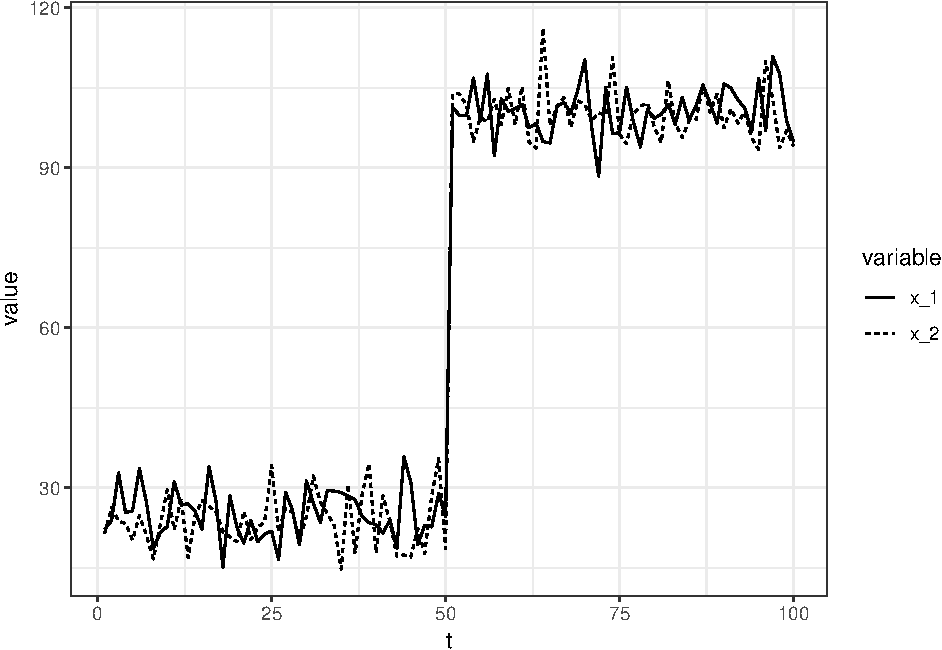
\includegraphics{_myDissertation_files/figure-latex/sysEx-1.pdf}
\caption{\label{fig:sysEx}The 2-variable toy system used to demonstrate steps for calculating system velocity. Each variable, \(x\), is drawn from a normal distribution with means that change at \(t = 50\). State variables have constant variance \(\sigma = 5\).}
\end{figure}
\hypertarget{steps-for-calculating-system-velocity-v}{%
\subsection{\texorpdfstring{Steps for calculating system velocity, \(v\)}{Steps for calculating system velocity, v}}\label{steps-for-calculating-system-velocity-v}}

First, we calculate the change in each state variable, \(x_i\), between two adjacent points in time, \(t_j\) and \(t_{j+1}\), such that the difference, \(x_{t_{j+1}} - x_{t_j}\) is assigned to the latter time point, \(t_{j+1}\). For example, in our toy data, we use observations at time points \(t = 1\) \& \(t=2\) (Fig. \ref{fig:sysEx2}). For all examples in this chapter, the state variables \(x_1\) and \(x_2\) were drawn from a normal distribution (using function \emph{rnorm}), with parameters \(\bar{x}_i\) (mean) and \(\sigma_i\) (sd) for 100 time steps, \(t\). The regime shift occurs at \(t=50\), where a shift in either or both \(\bar{x}_i\) or \(\sigma_i\).

\hypertarget{step-1-delta-x_i}{%
\subsubsection{\texorpdfstring{Step 1: \(\Delta x_i\)}{Step 1: \textbackslash{}Delta x\_i}}\label{step-1-delta-x_i}}

The first step in calculating \(v\) is to obtain the change in values for each state variables, \(x_1\) and \(x_2\) between two consecutive time points (e.g., from \(t=1\) to \(t=2\):
\begin{equation}
\begin{array}{rcr}
\Delta x_1 = x_{1_{t=2}} - x_{1_{t=1}} \\
\Delta x_2 = x_{2_{t=2}} - x_{1_{t=1}}
  \end{array}
\label{eq:diffX}
\end{equation}
\begin{Shaded}
\begin{Highlighting}[]
\NormalTok{p.sysEx }\OperatorTok{+}
\StringTok{  }\KeywordTok{geom_point}\NormalTok{(}\DataTypeTok{data =}\NormalTok{df, }\KeywordTok{aes}\NormalTok{(}\DataTypeTok{x =}\NormalTok{ t, }\DataTypeTok{y =}\NormalTok{ value, }\DataTypeTok{shape =}\NormalTok{ variable, }\DataTypeTok{color=}\NormalTok{variable), }\DataTypeTok{size=}\DecValTok{4}\NormalTok{)}\OperatorTok{+}
\StringTok{  }\KeywordTok{xlim}\NormalTok{(}\KeywordTok{c}\NormalTok{(}\DecValTok{1}\NormalTok{,}\DecValTok{2}\NormalTok{))}\OperatorTok{+}\KeywordTok{ylim}\NormalTok{(}\KeywordTok{c}\NormalTok{(}\DecValTok{20}\NormalTok{,}\DecValTok{30}\NormalTok{))}\OperatorTok{+}
\StringTok{  }\KeywordTok{scale_color_manual}\NormalTok{(}\DataTypeTok{values=}\KeywordTok{c}\NormalTok{(}\StringTok{"red"}\NormalTok{,}\StringTok{"black"}\NormalTok{))}\OperatorTok{+}
\StringTok{  }\KeywordTok{theme}\NormalTok{(}\DataTypeTok{legend.position =} \StringTok{'bottom'}\NormalTok{)}\OperatorTok{+}
\StringTok{  }\KeywordTok{theme_bw}\NormalTok{()}
\end{Highlighting}
\end{Shaded}
\begin{verbatim}
Warning: Removed 196 rows containing missing values (geom_path).
\end{verbatim}
\begin{verbatim}
Warning: Removed 196 rows containing missing values (geom_point).
\end{verbatim}
\begin{figure}
\centering
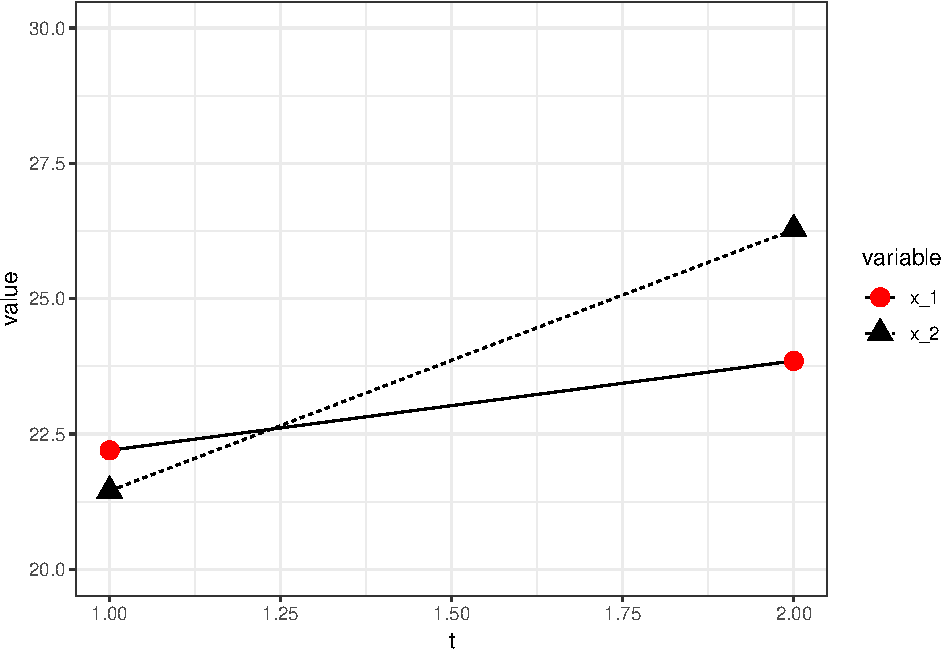
\includegraphics{_myDissertation_files/figure-latex/sysEx2-1.pdf}
\caption{\label{fig:sysEx2}Data used to calculate velocity at the first two time points, \(t_1\) and \(t_2\).}
\end{figure}
\hypertarget{step-2-sqrtsum_indelta-x_12}{%
\subsubsection{\texorpdfstring{Step 2: \(\sqrt(\sum_i^N\Delta x_1^2)\)}{Step 2: \textbackslash{}sqrt(\textbackslash{}sum\_i\^{}N\textbackslash{}Delta x\_1\^{}2)}}\label{step-2-sqrtsum_indelta-x_12}}

After calculating the differences for each state variable, we will next calculate the total change in the system over the time elapsed, following Pythagora's theorem,
\begin{equation}
 X_1^2 + X_2^2 = s^2 
  \label{eq:pythagorean}
\end{equation}
where \(s\) represents the total change in the system, and \(X_1\) and \(X_2\) represent the changes in all state variables (\(x_{i_{t=2}} - x_{i_{t=1}}\)). We achieve this by first squaring the differences obtained in Eq. \eqref{eq:diffX}:
\begin{equation}
\begin{array}{rcr}
(x_{1_{t=2}} - x_{1_{t=1}})^2  \\
(x_{2_{t=2}} - x_{2_{t=1}})^2 
\end{array}
  \label{eq:diffXsq}
\end{equation}
\hypertarget{step-3-use-pythagorean-theorem-to-isolate-s}{%
\subsubsection{\texorpdfstring{Step 3: Use Pythagorean theorem to isolate \(s\)}{Step 3: Use Pythagorean theorem to isolate s}}\label{step-3-use-pythagorean-theorem-to-isolate-s}}

Next, we isolate \(s\) in Eq. \eqref{eq:pythagorean}, capturing the total change in all state variables into a single measure by taking the 2nd root of the squared sums of all \(x\):
\begin{equation}
\begin{array}{rcr}
\sum_{i=1}^{N} \Delta {x_i} = \sum_{i=1}^{N}(x_{t_{i+1}} - x_{t_i})^2 \\ 
\ = \Delta s \\ 
\ = \sqrt([x_{1_{t=2}} - x_{1_{t=1}}]^2 + [x_{2_{t=2}} - x_{2_{t=1}}]^2)
\end{array}
\label{eq:diffXsq2}
\end{equation}
We now have a single measure, \(\Delta s\) (Eq. \eqref{eq:diffXsq2}), for each pair of time points in our \(N\)-dimensional system. It is obvious that \(\Delta s\) will always be a positive value, since we took the 2nd root of a squared value. Although discussed in a later section, it is important to note that this value is not unitless--that is, our example system takes on the units of our state variables, \(x_1\) and \(x_2\). Because we are interested in identifying abrupt changes in the entire system, we calculate the cumulative sum of \(\Delta s\) at every time point, such that:
\begin{equation}
s = \sum_{t=1}^T \Delta s
\label{eq:s}
\end{equation}
\hypertarget{rRDM}{%
\chapter*{Appendix A}\label{rRDM}}
\addcontentsline{toc}{chapter}{Appendix A}

Placeholder

\hypertarget{references}{%
\chapter*{References}\label{references}}
\addcontentsline{toc}{chapter}{References}

Placeholder

\hypertarget{refs}{}
\leavevmode\hypertarget{ref-fath_regime_2003}{}%
Fath, B. D., Cabezas, H., \& Pawlowski, C. W. (2003). Regime changes in ecological systems: An information theory approach. \emph{Journal of Theoretical Biology}, \emph{222}(4), 517--530. \url{http://doi.org/10.1016/S0022-5193(03)00067-5}


\end{document}
